\chapter{MATERIALES Y MÉTODOS}
% https://drive.google.com/drive/u/1/folders/1HxnrVCsACM1mNTN5ifr0aDUULJwfmJMG
\section{Descripción del lugar de ejecución}
El proyecto será ejecutado en oficina de CONCYTEC - UPeU. El lugar es elegido porque ésta investigación es parte del proyecto “Plataforma digital inteligente y Big Data para el turismo rural comunitario en la Región Puno”.
\section{Materiales e insumos}
%Técnicas de investigación, instrumentos(materiales)
Los materiales a usar en el desarrollo de este proyecto más importantes se muestran en la tabla \ref{tab:materiales}:
\begin{table}[ht]
\caption{Materiales e insumos}
\label{tab:materiales}
\begin{tabular}{ll} \hline
\textbf{Herramienta} &\textbf{Descripción}\\ \hline
 Python(3.7) & Lenguaje de programación \\
 Django(2.1) & Framework web de python \\
 Sqlite & Base de datos relacional \\
 Api Google Maps & Servidor de aplicaciones de mapas en la web \\ 
 PyCharm(2018.2.4) & Entorno de desarrollo integrado para python \\
 \hline
\end{tabular}
\end{table}

\section{Metodología}
\subsection{Tipo de investigación}
El presente trabajo de investigación se encuentra dentro de una investigación tecnológica porque esta en el ámbito de producción tecnológica, investigación aplicativa, también propositiva por lo siguiente:
\begin{itemize}[noitemsep]
    \item Teoría: Optimización multiobjetivo
    \item Hecho: Diseñar viajes personalizados
    \item Solución: Implementar modelo
\end{itemize}
%\subsection{Arquitectura de la solución}

\subsection{Metodología de la investigación}
La metodología que se usará es el de investigación de operaciones mencionado en el marco teórico desde el enfoque de la solución al modelo de inteligencia artificial en la construcción un algoritmo metaheuristico. Para las dos primeras fases se tomará de un modelo propuesto por \citeA{RodriguezDiaz2012SistemaPersonalizado} realizado en Andalucía (España), esta propuesta es tomada porqué como hay un trabajo realizado en otro lugar, se pretende implementar el mismo modelo, pero como puede variar de acuerdo al lugar, se pretende ajustar al tener los datos e implementar. Para la tercera fase de construcción se considerará dos primeros objetivos por el énfasis que se dará en la construcción del algoritmo y cuarta fase se corresponderá al tercer objetivo, así sucesivamente.
\subsubsection{Diagrama de flujo de las actividades de la investigación}
El diagrama de flujo de las actividades de la presente investigación se muestra en la figura \ref{fig:fases_investigacion}.

\begin{figure}[!ht]
    \centering
    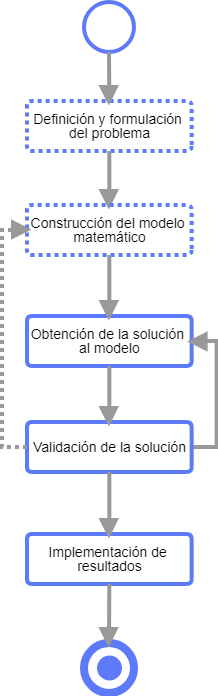
\includegraphics[scale=.5]{Capitulo4/Figs/fases_investigacion.png}
    \caption{Diagrama de flujo de las actividades de la investigación}
    \label{fig:fases_investigacion}
\end{figure}
%\subsubsection{Arquitectura de solución}
\begin{figure}[!ht]
    \centering
    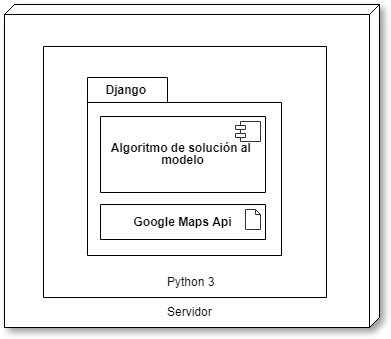
\includegraphics[scale=.5]{Capitulo4/Figs/aquitectura_solucion.png}
    \caption{Diagrama de la arquitectura de solución de la investigación}
    \label{fig:aquitectura_solucion}
\end{figure}

\subsubsection{Objetivo 1}
Desarrollar el algoritmo de heurística de construcción El vecino más cercano y la heurística de mejoría 2-opt y/o otros, utilizando el lenguaje de programación Python.

\paragraph{Metodología}
Para implementar se tomará el código realizado por \citeA{mendoza2017diseno}.
%De acuerdo a la teoría de algoritmos con la que se tiene relación se implementara los diagramas de flujo para una mejor comprensión del algoritmo.
%Se ajustarán los algoritmos de heurística de construcción y mejoría diseñados por \citeA{mendoza2017diseno} de acuerdo al modelo matemático ref. en el lenguaje de programación Python.

%Resultado esperado
\subsubsection{Objetivo 2}
Desarrollar el algoritmo de metaheurística Búsqueda Tabú para mejorar la solución de la heurística de mejoría, utilizando Python.
\paragraph{Metodología.}
Para implementar se tomará el código realizado por \citeA{mendoza2017diseno} y se ajustará de acuerdo al modelo.
\subsubsection{Objetivo 3}
Validar el algoritmo con técnicas estadísticas utilizando instancias artificiales encontradas en la literatura y/o de datos simulados, y datos reales de la región Puno.
\paragraph{Metodología}
Primeramente en el objetivo 2 se trabajará con datos simulados, luego se recolectaran los datos reales para el ajuste del modelo y la construcción del algoritmo, luego de implementarse se buscarán instancias artificiales para validar usando técnicas estadísticas.
\subsubsection{Objetivo 4}
Desarrollar una aplicación web que permita al turista ingresar sus preferencias y visualizar el itinerario detallado utilizando el framework web Django y Api de Google Maps.
\paragraph{Metodología}
Se usará la metodología de desarrollo Programación Extrema.
%Se implementará una aplicación web con la metodología de ...,en la que considerará 

%La metodología debe escribirse en forma detallada y por cada objetivo. Debe incluir la cita respectiva de los autores que han propuesto el método. La descripción de métodos debe considerar lo siguiente: a) Frecuencia temporal requerida para la toma de datos. b) Materiales y equipos a ser utilizados. c) Variables a ser analizadas. (si fuera el caso) d) Prueba(s) estadística(s) que se utilizará(n) para probar las hipótesis. (si fuera el caso)
